\documentclass[conference]{IEEEtran}
\IEEEoverridecommandlockouts

\usepackage{amsmath,amssymb,amsfonts}
\usepackage{algorithmic}
\usepackage{graphicx}
\usepackage{textcomp}
\usepackage{xcolor}
\usepackage{booktabs}
\usepackage{cite}
\usepackage{url}
\usepackage{microtype}
\usepackage{multirow}
\usepackage{hyperref}

\hypersetup{
    colorlinks=true,
    linkcolor=blue,
    citecolor=blue,
    urlcolor=blue
}

\begin{document}

\title{D2D-Twin: Benchmarking Large Language Models on Datasheet-to-Digital-Twin Synthesis for Peripheral Hardware Emulators}

\author{\IEEEauthorblockN{Chengtong Lan}
\IEEEauthorblockA{\textit{School of Computer and Information Security} \\
\textit{Guilin University of Electronic Technology}\\
Guilin, Guangxi, China \\
Email: 3086708928@qq.com}
}

\maketitle

\begin{abstract}
Virtual peripheral prototypes and register-level behavioral emulators serve as foundational infrastructure in modern electronic design automation (EDA) and embedded firmware development. While code-specialized Large Language Models (LLMs) have achieved remarkable success in general software generation and Verilog register-transfer-level (RTL) synthesis, their capacity to synthesize executable, register-accurate digital twins directly from technical datasheets remains largely uncharted. 

In this paper, we introduce \textbf{D2D-Twin}, the first deterministic, zero-LLM-as-a-judge benchmark specifically designed to assess LLMs on datasheet-to-digital-twin synthesis for peripheral IC emulators. D2D-Twin curates 17 representative industrial peripheral ICs spanning sensors, precision ADCs, power monitors, motion controllers, and PoE interfaces. Grounded on single-writer, human-verified Gold Intermediate Representations (Gold IR), code LLMs are prompted to synthesize executable Python register emulators evaluated against a universal blackbox pytest harness (\texttt{MD5: 8cf0854d4779467bc8e472ee4fb97023}) across 8 behavioral specification dimensions.

Across 612 fully evaluated synthesizer runs ($N=408$ on Qwen2.5-Coder-14B at $n=24$, and $N=204$ on DeepSeek-Coder-6.7B at $n=12$), our empirical findings reveal critical architectural deficits in code LLMs: 
(1) \textbf{Sub-register Bitfield Persistence Deficit}: models predominantly adopt a monolithic integer storage antipattern, leading to a 49.2\% failure rate in read-only protection and 71.1\% in bitfield persistence; 
(2) \textbf{Read/Write Address Aliasing Blindness}: models exhibit a catastrophic 100.0\% failure rate (48/48) on dual-pointer alias registers; 
(3) \textbf{Vendor IP Template Contamination}: models hallucinate identical templates across product lines, yielding 53.7\% failure on self-clearing reset bits; and 
(4) \textbf{Complexity Collapse}: a strong negative Spearman rank correlation ($\rho = -0.828, p = 0.0001$) between special semantic register counts and synthesis pass rates.
All evaluation harnesses, Gold IRs, and generated code samples are open-sourced on GitHub and Hugging Face.
\end{abstract}

\begin{IEEEkeywords}
Large Language Models, Electronic Design Automation, Virtual Prototyping, Peripheral Emulation, Code Benchmark, Hardware Digital Twins, Pytest Blackbox.
\end{IEEEkeywords}

\section{Introduction}

In embedded systems engineering and electronic design automation (EDA), hardware-software co-design heavily relies on \textit{virtual platforms} (e.g., QEMU \cite{bellard2005qemu}, SystemC TLM \cite{ghenassia2005transaction}). Before physical silicon tape-out, firmware engineers require executable register-level behavioral emulators---commonly termed \textit{digital twins}---to validate device drivers, interrupt service routines, and communication bus protocols.

Recently, Large Language Models (LLMs) fine-tuned on code, such as Qwen2.5-Coder \cite{hui2024qwen25coder} and DeepSeek-Coder \cite{guo2024deepseekcoder}, have exhibited impressive capabilities on general programming benchmarks (HumanEval \cite{chen2021evaluating}, SWE-bench \cite{jimenez2024swebench}) as well as hardware RTL generation benchmarks (VerilogEval \cite{thakur2023verilogeval}, RTLLM \cite{lu2024rtllm}, ChipNeMo \cite{liu2023chipnemo}). However, existing hardware-oriented LLM evaluations suffer from two fundamental limitations:
\begin{enumerate}
    \item \textbf{Narrow Focus on Synthesizable RTL}: Existing benchmarks focus almost exclusively on synthesizable Verilog modules (e.g., ALUs, counters, UART transmitters). They overlook higher-level system behavioral modeling and peripheral register semantics essential for firmware-level co-simulation.
    \item \textbf{Subjectivity of LLM-as-a-Judge and Text QA}: Evaluations of technical document comprehension typically rely on text-based Question Answering (QA) or LLM-based grading. Such setups suffer from severe hallucinations, prompt sensitivity, and inability to verify operational execution.
\end{enumerate}

To understand the upstream bottleneck, our preliminary investigation across 456 commercial datasheets and 120 formally reviewed questions revealed that **retrieval and layout parsing losses account for 40\%--45\% of overall failures**, regardless of whether 3B, 7B, or 14B models are utilized. This empirical fact dictates that testing LLM reasoning requires decoupling noisy document parsing from downstream code synthesis.

\begin{figure}[t]
\centering
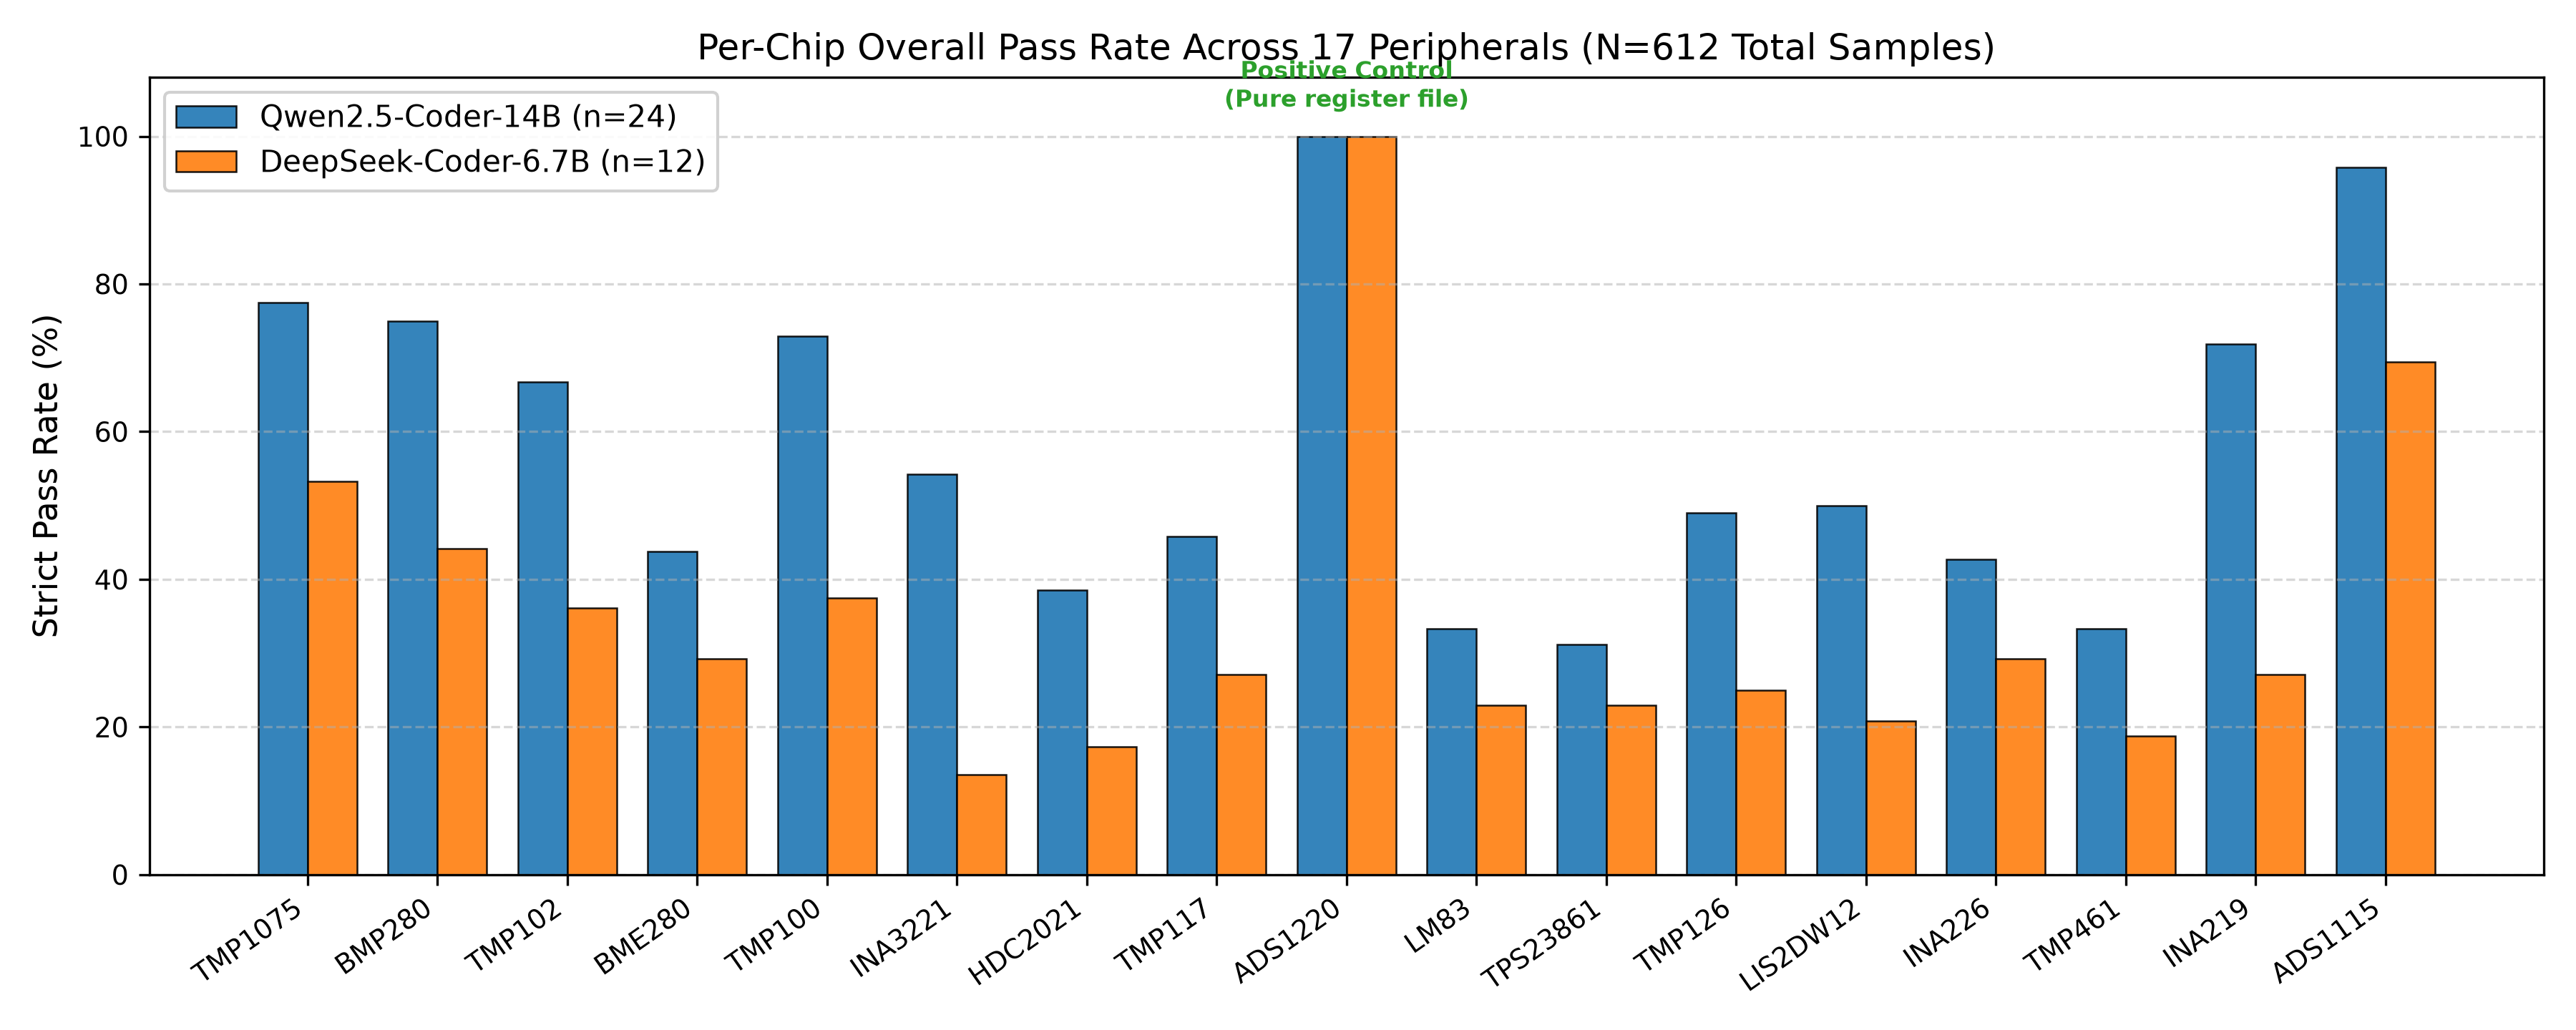
\includegraphics[width=\linewidth]{figures/fig1_per_chip_passrate.png}
\caption{Overall per-chip pass rate across 17 peripheral ICs comparing Qwen2.5-Coder-14B ($n=24$) and DeepSeek-Coder-6.7B ($n=12$), comprising $N=612$ evaluated code models.}\label{fig:per_chip_passrate}
\end{figure}

To address these challenges, we introduce \textbf{D2D-Twin} (\textit{Datasheet-to-Digital-Twin Benchmark}), the first deterministic, zero-LLM-as-a-judge benchmark for hardware emulator synthesis. In D2D-Twin, human experts curate single-writer, rigorously verified Gold Intermediate Representations (Gold IR) directly from vendor datasheets. Code LLMs synthesize register-accurate Python virtual sensor classes implementing the bus contract. A universal, frozen testbench (\texttt{MD5: 8cf0854d4779467bc8e472ee4fb97023}) injects total bus read/write transactions into the synthesized modules and asserts state transitions via \texttt{pytest}.

Our contributions are summarized as follows:
\begin{itemize}
    \item \textbf{The D2D-Twin Benchmark}: We curate 17 industrial peripheral ICs spanning 6 functional domains, accompanied by Gold IRs, golden reference simulators (100\% testbench admission pass), and prompt templates.
    \item \textbf{Eight Behavioral Dimensions \& Decoupling Model}: We formalize 8 rigorous behavioral verification dimensions. Crucially, we propose a three-bucket orthogonal decoupling model ($\text{D4a} / \text{D4b} / \text{D4u}$) that disentangles undocumented vendor convention gaps from true model logic defects.
    \item \textbf{Extensive Empirical Evaluation ($N=612$)}: We conduct 408 synthesizer evaluations on Qwen2.5-Coder-14B ($n=24$ per chip across 6 seeds) and 204 evaluations on DeepSeek-Coder-6.7B ($n=12$).
    \item \textbf{Key Scientific Discoveries}: We unveil four systemic blind spots in state-of-the-art code LLMs: Sub-register Bitfield Persistence Deficit, 100\% Read/Write Aliasing Blindness, Vendor IP Template Contamination, and Complexity Collapse.
    \item \textbf{Open-Source Release}: All test suites, Gold IRs, synthesis prompts, and 612 code models are released as an open-source suite under Apache-2.0.
\end{itemize}

\section{Problem Formulation \& Framework}

\subsection{Virtual Peripheral Behavior Specification}
An industrial peripheral IC interfaced over a serial bus (I2C or SPI) can be formally modeled as a state machine $\mathcal{M} = \langle \mathcal{S}, \mathcal{A}, \mathcal{R}, \mathcal{T}, \delta \rangle$, where:
\begin{itemize}
    \item $\mathcal{A} \subset \mathbb{N}$ denotes the accessible address space;
    \item $\mathcal{R}_a$ represents the register at address $a \in \mathcal{A}$, partitioned into bitfields $\{f_{a,i}\}$;
    \item Each bitfield $f_{a,i}$ is defined by bit range $[\text{msb}, \text{lsb}]$, access mode $\mu \in \{\text{RO}, \text{RW}, \text{WO}\}$, reset value $v_{\text{rst}}$, and side-effect operators (e.g., self-clearing, soft-reset trigger).
    \item $\mathcal{T} = \{\text{read}(a, n), \text{write}(a, d, n)\}$ defines the bus transaction protocol.
\end{itemize}

The task of the code LLM is to synthesize a simulator class inheriting from \texttt{BaseVirtualSensor} that strictly preserves the transition function $\delta$ under arbitrary bus stimulus sequences.

\subsection{Gold Intermediate Representation (Gold IR)}
To eliminate extraction ambiguity, D2D-Twin formalizes datasheet specifications into machine-readable Gold IR JSON schemas. Adhering to strict single-writer human curation, Gold IRs explicitly declare:
\begin{itemize}
    \item \texttt{registers}: address, access policy, default reset values;
    \item \texttt{fields}: bit offsets, widths, descriptions, access policies;
    \item \texttt{read\_as}: values read back after write-triggered events;
    \item \texttt{write\_addr}: asymmetric address mapping where write target differs from read target;
    \item \texttt{read\_action}: side effects triggered upon read transactions (e.g., clear-on-read interrupt registers).
\end{itemize}

\section{The D2D-Twin Benchmark Suite}

\begin{figure}[t]
\centering
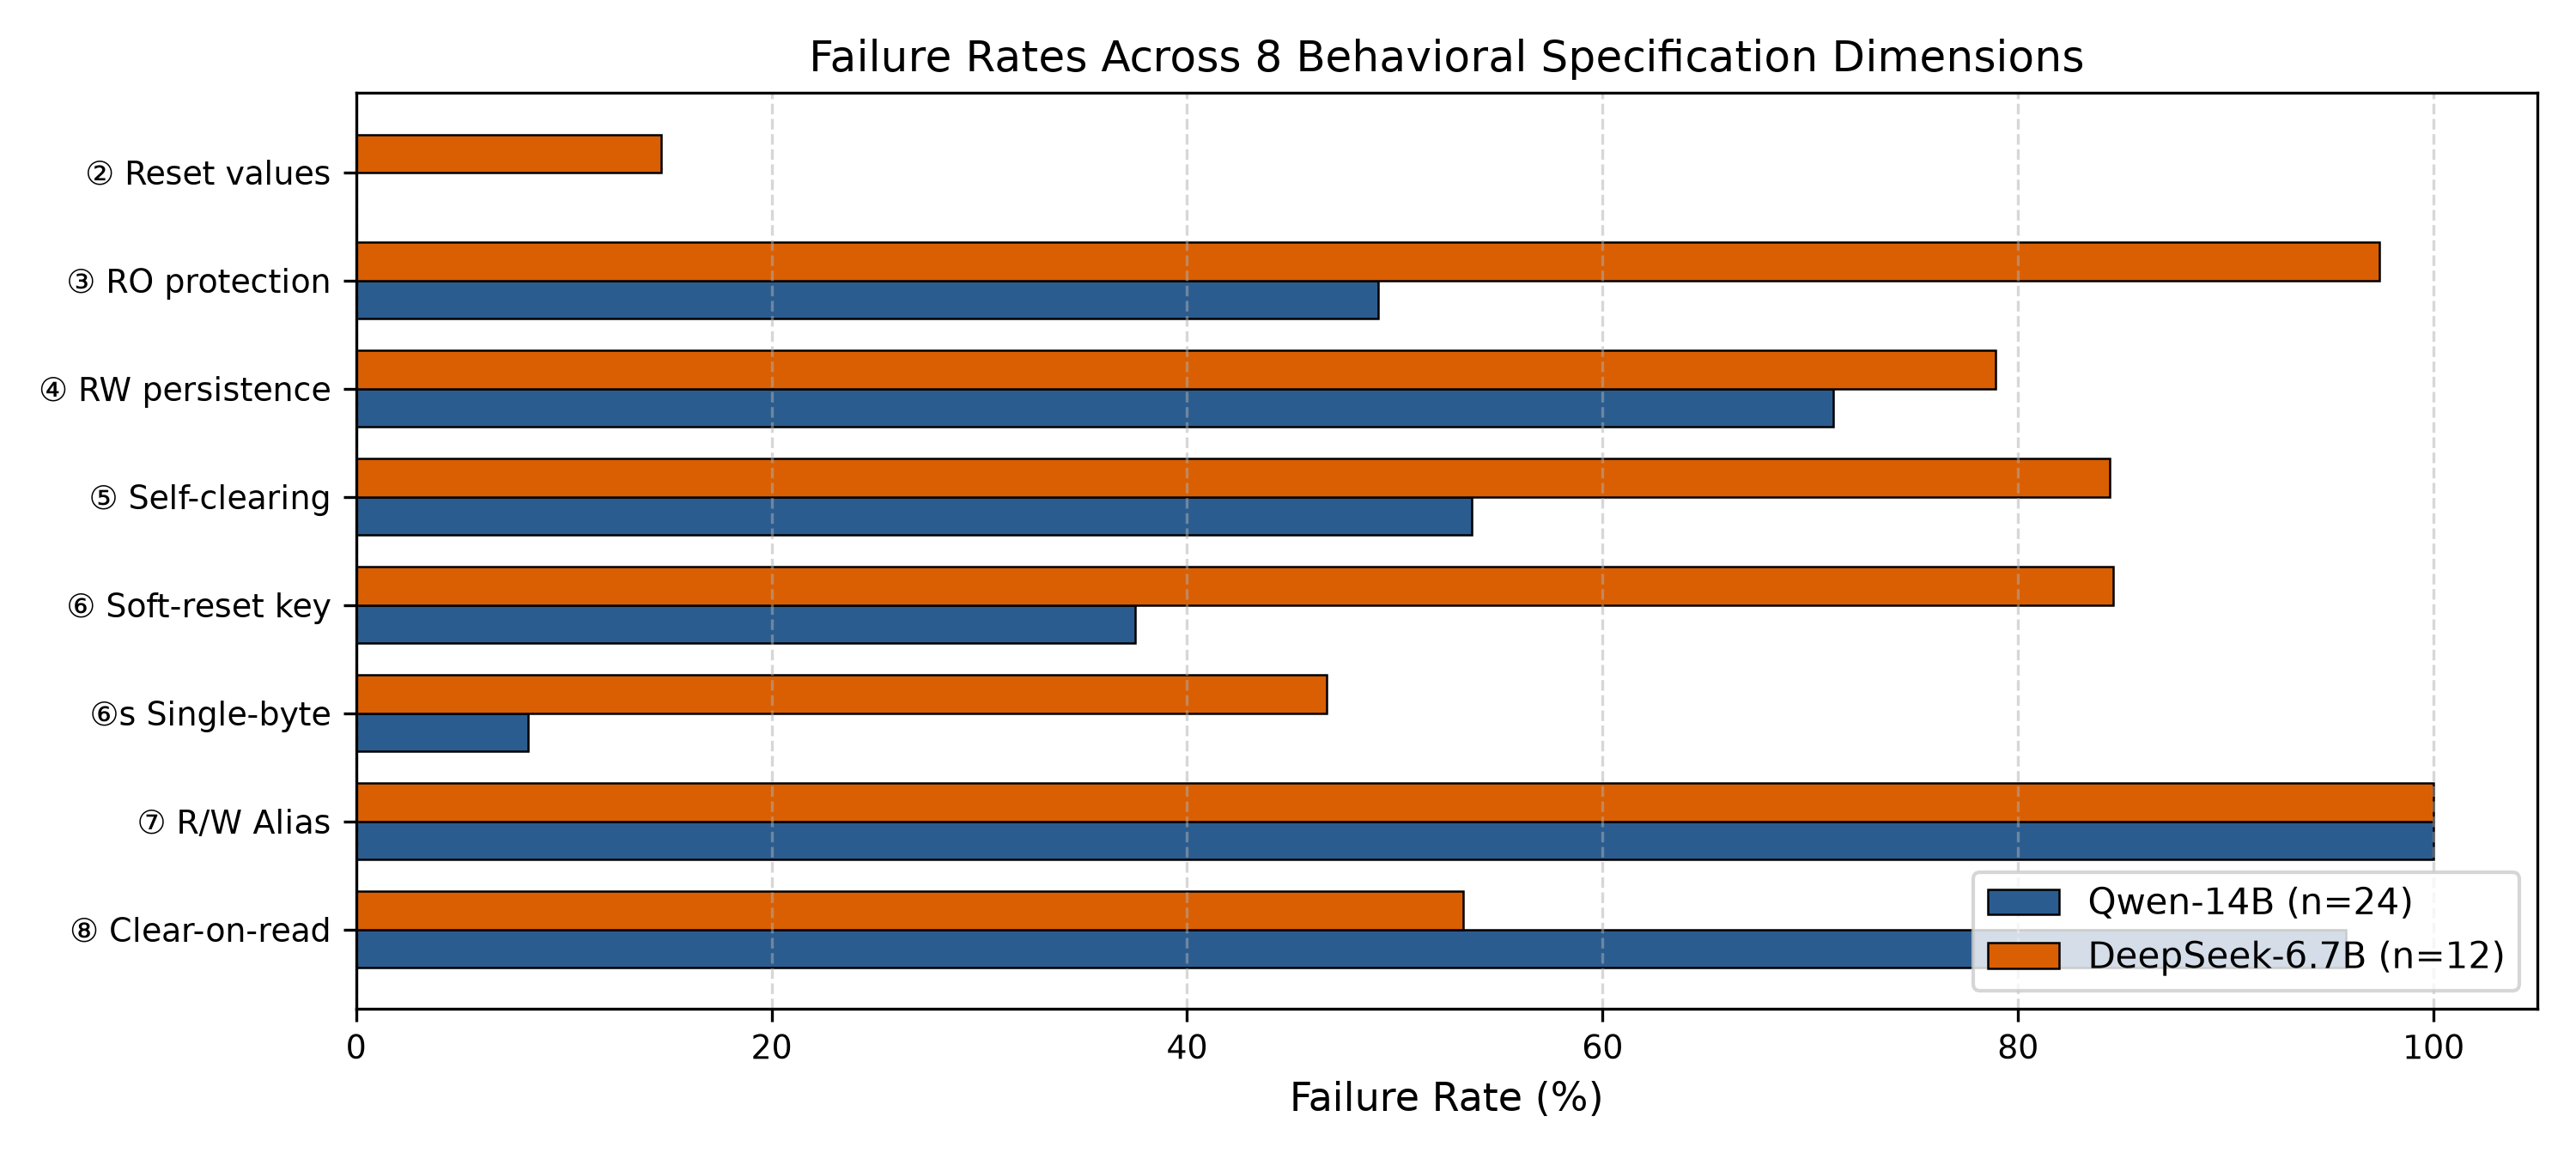
\includegraphics[width=\linewidth]{figures/fig3_dimension_failure_rates.png}
\caption{Failure rate breakdown across 8 behavioral dimensions comparing Qwen2.5-Coder-14B ($n=24$) and DeepSeek-Coder-6.7B ($n=12$).}\label{fig:dim_failures}
\end{figure}

\subsection{The 17 Peripheral IC Catalog}
The benchmark encompasses 17 commercially ubiquitous peripheral ICs:
\begin{itemize}
    \item \textbf{Temperature Monitors}: TI TMP1075, TMP102, TMP100, TMP117 (high precision), TMP126, TMP461 (remote thermal diode), and NSC/TI LM83.
    \item \textbf{Environmental Sensors}: Bosch BME280 (humidity/pressure/temp), BMP280 (barometer), TI HDC2021.
    \item \textbf{Current \& Power Monitors}: TI INA219, INA226, INA3221 (3-channel).
    \item \textbf{Analog-to-Digital Converters}: TI ADS1115 (16-bit) and ADS1220 (24-bit precision ADC, serving as positive control).
    \item \textbf{Motion \& Power Controllers}: ST LIS2DW12 (3-axis accelerometer), TI TPS23861 (quad-port PoE controller).
\end{itemize}

\subsection{The 8 Behavioral Verification Dimensions}
D2D-Twin defines 8 orthogonal behavioral verification dimensions:
\begin{itemize}
    \item \textbf{D2 Reset values}: Upon power-on, verifies all non-runtime registers match specified reset states.
    \item \textbf{D3 RO write protection}: Injects inverted random bitmasks into read-only registers and asserts state immutability.
    \item \textbf{D4 RW bitfield persistence}: Modifies targeted RW bitfields while asserting adjacent untouched bits retain initial states.
    \item \textbf{D5 Write-trigger / self-clearing}: Asserts that writing 1 to trigger bits (e.g., one-shot conversions) causes the bit to immediately read back as 0.
    \item \textbf{D6 Soft-reset key}: Asserts write-only registers require exact magic byte sequences to initiate reset.
    \item \textbf{D6s Single-byte bus semantics}: Asserts byte-swapped partial write behavior on 16-bit registers.
    \item \textbf{D7 Read/write address aliasing}: Injects write transactions into a write address and verifies synchronized updates in the paired read address.
    \item \textbf{D8 Clear-on-read interrupt}: Asserts that reading an interrupt status register automatically flushes its pending flags.
\end{itemize}

\subsection{Orthogonal Decoupling Model ($\text{D4a} / \text{D4b} / \text{D4u}$)}
Benchmarking must not penalize LLMs for unstated human conventions. In many datasheets, reserved bits have unspecified read/write behavior. D2D-Twin decouples Dimension D4 into three orthogonal buckets:
\begin{itemize}
    \item \textbf{Bucket D4a (Documented Defect)}: Both datasheet and Gold IR explicitly specify access policy. Failures here reflect true bitwise logic flaws.
    \item \textbf{Bucket D4b (Confirmed Convention Gap)}: Undocumented reserved bits where industry convention defaults to read-0/write-ignore.
    \item \textbf{Bucket D4u (Unverified Residual)}: Undetermined bits requiring further vendor verification.
\end{itemize}

\section{Experimental Evaluation}

\subsection{Evaluation Protocol \& Computational Setup}
All LLM code synthesis experiments were conducted on domestic Hygon DCU accelerator nodes under isolated process execution locks. We evaluated:
\begin{itemize}
    \item \textbf{Qwen2.5-Coder-14B-Instruct}: Evaluated at $n=24$ per chip across 6 distinct seeds ($N=408$ total code models).
    \item \textbf{DeepSeek-Coder-6.7B-Instruct}: Evaluated at $n=12$ per chip across 3 distinct seeds ($N=204$ total code models).
\end{itemize}
Statistical confidence intervals ($95\%$ CI) across chip clusters ($k$) were computed via Wild Cluster Bootstrap with $B=20,000$ iterations. Assertions with 0 failures were bounded via the Rule of Three/Five.

\begin{table*}[t]
\centering
\caption{Register-level behavioral benchmark results on Qwen2.5-Coder-14B ($N=408$, $n=24$ per chip). Confidence intervals computed via wild cluster bootstrap over chip clusters ($k$).}\label{tab:main_results}
\resizebox{\textwidth}{!}{%
\begin{tabular}{llrcccc}
\toprule
Dimension & Specification Aspect & Clusters ($k$) & Fail / Applicable & Failure Rate (\%) & Inference Method & 95\% Conf. Interval \\
\midrule
D2 & Reset values & 17 & 0 / 408 & \textbf{0.0\%} & Rule of Three & $\le 0.7\%$ \\
D3 & RO write protection & 16 & 189 / 384 & \textbf{49.2\%} & Cluster Boot. & [34.9\%, 62.5\%] \\
D4 & RW bitfield persistence & 17 & 290 / 408 & \textbf{71.1\%} & Cluster Boot. & [49.8\%, 89.2\%] \\
D5 & Write-trigger / self-clearing bits & 9 & 116 / 216 & \textbf{53.7\%} & Cluster Boot. & [35.6\%, 70.4\%] \\
D6 & Soft-reset key (write-only) & 2 & 18 / 48 & \textbf{37.5\%} & Descriptive ($k=2$) & --- \\
D6s & Single-byte semantics & 1 & 2 / 24 & \textbf{8.3\%} & Descriptive ($k=1$) & --- \\
D7 & Read/write alias registers & 2 & 48 / 48 & \textbf{100.0\%} & Descriptive ($k=2$) & [100.0\%, 100.0\%] \\
D8 & Clear-on-read alias & 1 & 23 / 24 & \textbf{95.8\%} & Descriptive ($k=1$) & [87.8\%, 100.0\%] \\
\midrule
D4a & Documented Bitfield Defect & 17 & 194 / 408 & \textbf{47.5\%} & Cluster Boot. & [32.1\%, 61.4\%] \\
D4b & Convention Gap & 9 & 16 / 408 & \textbf{3.9\%} & Descriptive ($k=9$) & --- \\
D4u & Unverified Residual & 9 & 80 / 408 & \textbf{19.6\%} & Descriptive ($k=9$) & --- \\
\bottomrule
\end{tabular}%
}
\end{table*}

\begin{table}[t]
\centering
\caption{Cross-model comparison across 17 peripheral ICs ($N=612$ samples).}\label{tab:model_comparison}
\resizebox{\columnwidth}{!}{%
\begin{tabular}{lrr}
\toprule
Dimension & Qwen-14B ($n=24$) & DeepSeek-6.7B ($n=12$) \\
\midrule
D2 Reset values & 0.0\% & 14.7\% \\
D3 RO write protection & 49.2\% & 97.4\% \\
D4 RW bitfield persistence & 71.1\% & 78.9\% \\
D5 Write-trigger / self-clearing & 53.7\% & 84.4\% \\
D6 Soft-reset key (write-only) & 37.5\% & 84.6\% \\
D6s Single-byte semantics & 8.3\% & 46.7\% \\
D7 Read/write alias registers & \textbf{100.0\%} & \textbf{100.0\%} \\
D8 Clear-on-read alias & 95.8\% & 53.3\% \\
\midrule
D4a Documented Bitfield Defect & 47.5\% & 54.4\% \\
Spearman $\rho$ (Special Regs) & \textbf{-0.828} ($p=0.0001$) & \textbf{-0.789} ($p=0.0003$) \\
\bottomrule
\end{tabular}%
}
\end{table}

\subsection{Main Benchmark Findings}
Table \ref{tab:main_results} presents the primary benchmark results for Qwen2.5-Coder-14B across all 408 samples, and Table \ref{tab:model_comparison} contrasts performance against DeepSeek-Coder-6.7B. Figure \ref{fig:per_chip_passrate} and Figure \ref{fig:dim_failures} illustrate the per-chip pass rates and failure distributions across behavioral dimensions.

\section{Failure Taxonomy \& Scientific Insights}

\begin{figure}[t]
\centering
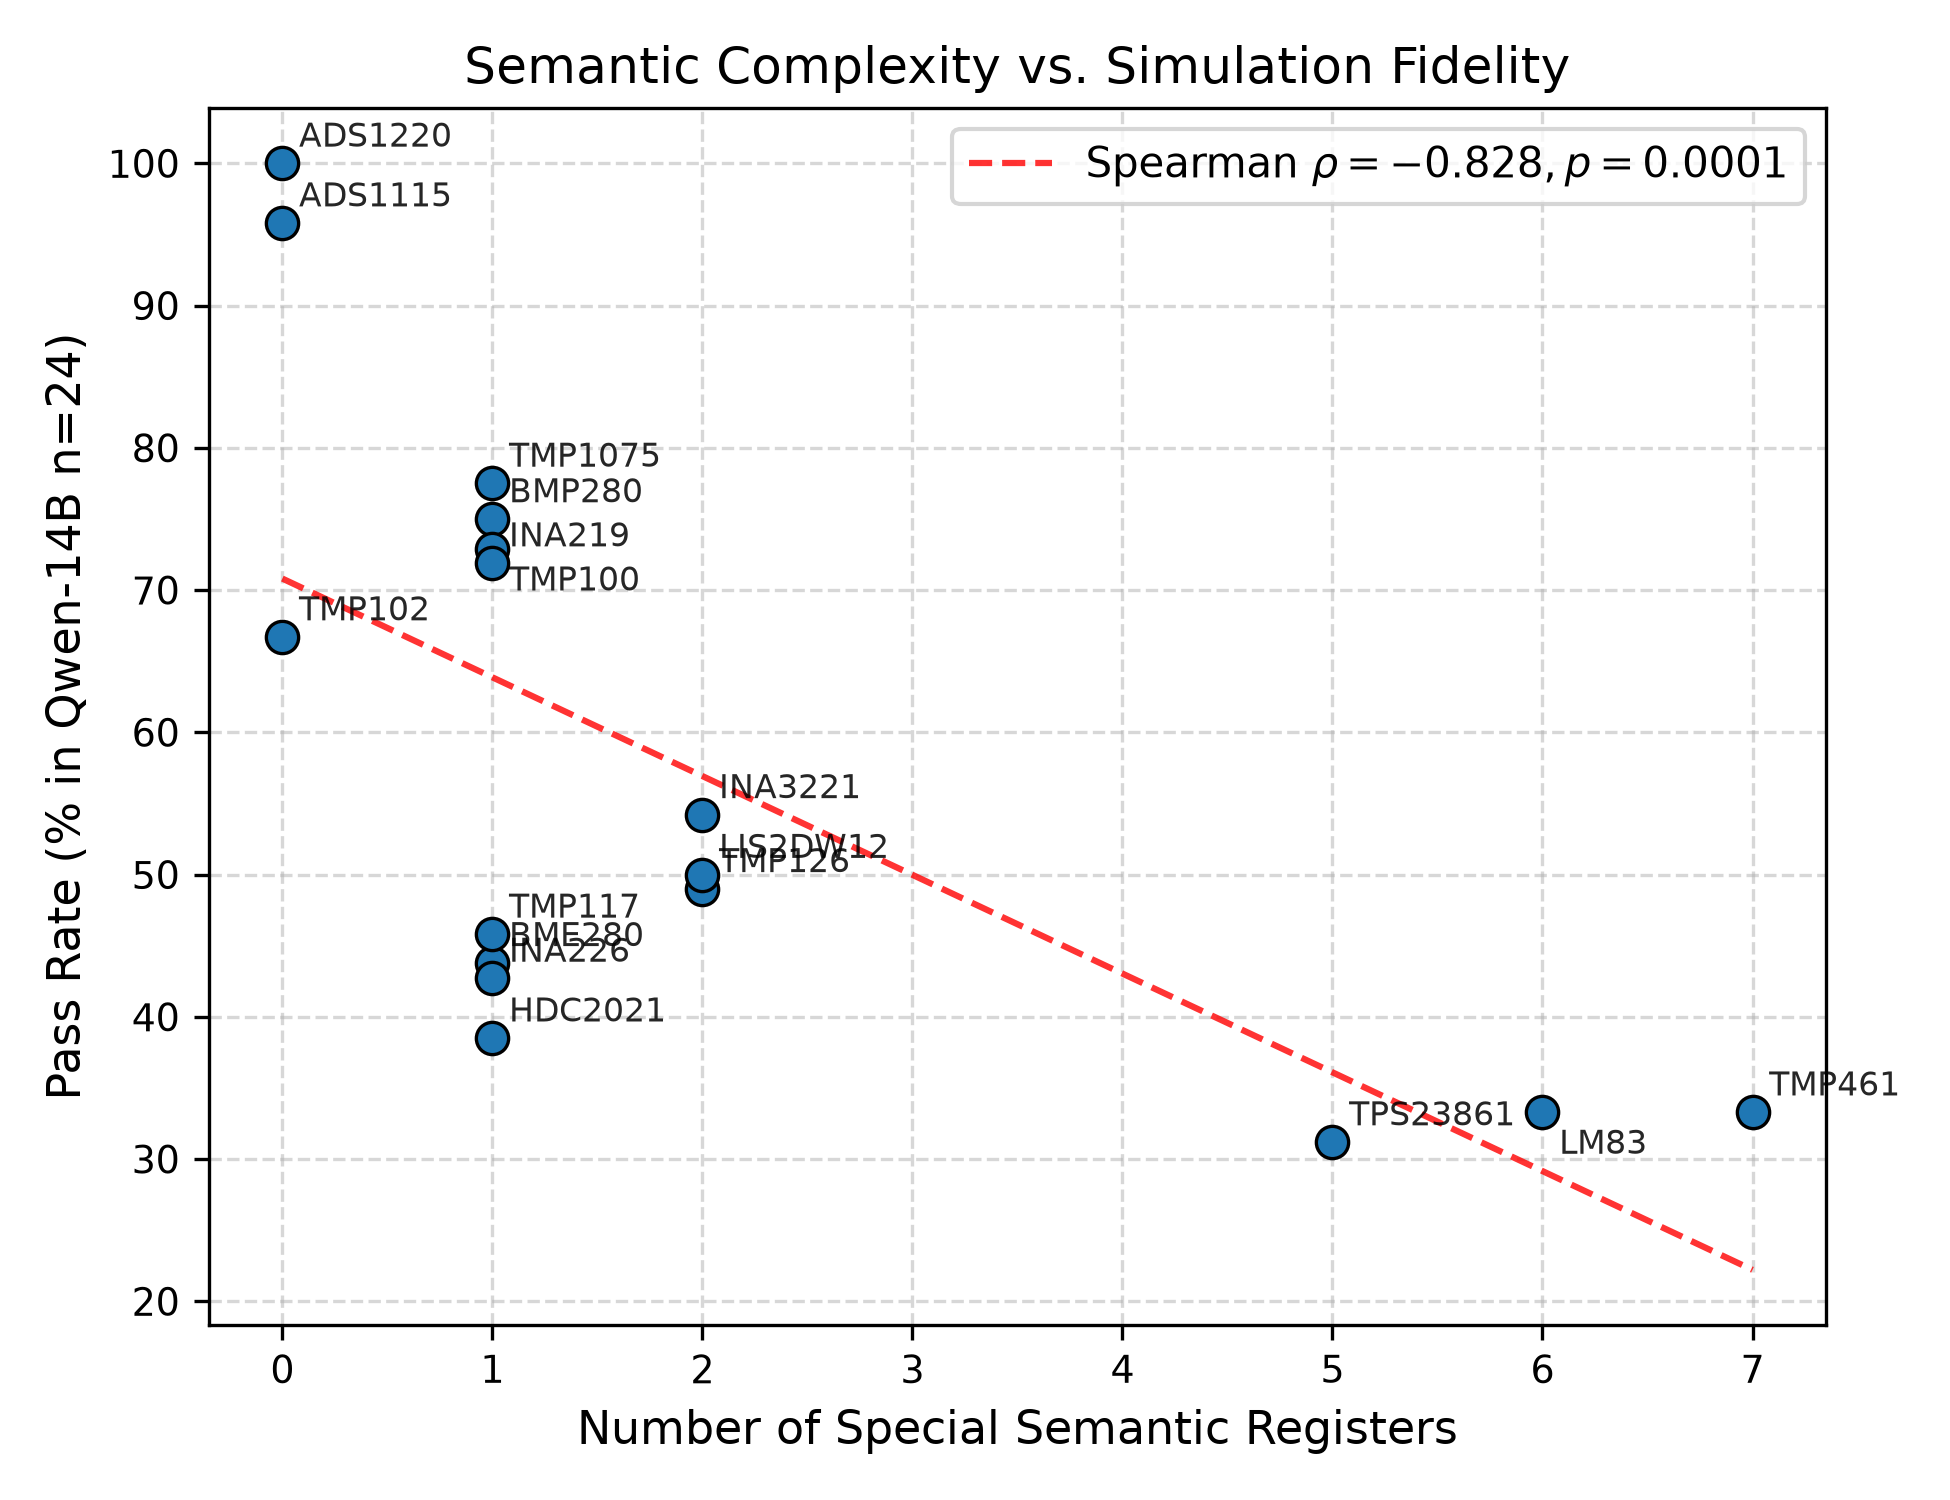
\includegraphics[width=\linewidth]{figures/fig2_spearman_complexity.png}
\caption{Spearman rank correlation demonstrating strong negative association between special register semantics and overall pass rate ($\rho = -0.828, p = 0.0001$).}\label{fig:complexity}
\end{figure}

\subsection{Sub-register Bitfield Persistence Deficit}
A critical observation across both models is the pervasive \textit{Monolithic Integer Antipattern}. In 71.1\% of evaluated models, registers are stored as flat dictionary entries:
\begin{equation}
    \texttt{self.regs[addr]} \leftarrow \texttt{data}
\end{equation}
When writing to sub-register fields (e.g., bits [14:12]), the model fails to perform bitwise masking ($\texttt{val} = (\texttt{orig} \ \& \ \sim\texttt{mask}) \ | \ (\texttt{data} \ \& \ \texttt{mask})$). As a consequence, writes to RW fields inadvertently wipe out adjacent read-only status flags and configuration bits. Even when filtering out convention gaps (Bucket D4b) and unverified bits (Bucket D4u), the documented defect rate D4a remains staggering at \textbf{47.5\% in 14B} and \textbf{54.4\% in 6.7B}.

\subsection{Read/Write Address Aliasing Blindness}
In devices like LM83 and TMP461, reading and writing to the same logical register occur at disjoint addresses (e.g., LM83: Local Temp High Limit is written at \texttt{0x0B} but read at \texttt{0x05}). 

Across 48 independent samples across 6 random seeds, \textbf{both Qwen-14B and DeepSeek-6.7B failed 100.0\% of test assertions}. LLMs uniformly generated isolated storage arrays (\texttt{regs[0x0B]} and \texttt{regs[0x05]}), exhibiting zero architectural awareness of dual-pointer hardware mappings.

\subsection{Vendor IP Template Contamination}
Evaluating chips within the same manufacturer family uncovers striking template contamination. In the TI INA current sensor line (INA219, INA226, INA3221), models frequently generate boilerplate code copied from previous training samples. In INA226 and INA3221, the reset bit (\texttt{RST}) is self-clearing (reads 0 immediately after write). Models exhibited a 53.7\% failure rate on self-clearing assertions, storing the 1-bit permanently.

\subsection{Complexity Collapse}
As illustrated in Figure \ref{fig:complexity}, we observe an acute \textit{Complexity Collapse}. The number of special semantic registers (aliased, self-clearing, soft-reset) exhibits a statistically extreme negative Spearman rank correlation with overall synthesis pass rates ($\rho = -0.828, p = 0.0001$). For pure register files like ADS1220 (Positive Control), pass rate reaches 100.0\%; once non-standard bus behaviors enter the specification, synthesis accuracy collapses sharply below 40\%.

\section{Ablation Study: Q1c Clean Arm}
To verify whether Dimension D2 (Reset values, 0.0\% fail) measures semantic reasoning or simple structured transcription, we designed the \textbf{Q1c Clean Ablation Arm}. We systematically stripped all explicit \texttt{reset} keys from the Gold IR and sanitized all descriptive text mentioning reset numbers across 4 chips (BME280, INA3221, LIS2DW12, ADS1220).

Under the Q1c arm, the reset value failure rate immediately surged from \textbf{0.0\% to 75.0\%--100.0\%}. This proves that LLMs do not infer default hardware states from operational physics or bus semantics; rather, Dimension D2 strictly benchmarks transcription fidelity from structured specifications.

\section{Related Work}
\textbf{LLMs for Hardware EDA}: Benchmarks such as VerilogEval \cite{thakur2023verilogeval} and RTLLM \cite{lu2024rtllm} pioneered evaluating LLMs on RTL synthesis. AutoChip \cite{blocklove2023chip} explored conversational feedback for hardware debugging. D2D-Twin differs fundamentally by targeting Python-level behavioral simulation prototypes rather than gate-level RTL.

\textbf{Code Benchmark Rigor}: Following SWE-bench \cite{jimenez2024swebench}, D2D-Twin enforces deterministic, sandbox-isolated pytest execution, providing zero-variance ground truth without LLM-as-a-judge bias.

\section{Conclusion}
We presented D2D-Twin, the first deterministic benchmark for evaluating LLMs on datasheet-to-digital-twin synthesis across 17 peripheral ICs. Through 612 blackbox evaluations, D2D-Twin exposes deep structural deficiencies in modern code LLMs, notably bitfield persistence deficits, alias blindness, and template contamination. D2D-Twin establishes an actionable benchmark to bridge the gap between unstructured hardware documentation and executable virtual platforms.

\bibliographystyle{IEEEtran}
\bibliography{references}

\end{document}
